\subsection{Mastering the Smith Chart: Normalization Made Easy!}

\begin{tcolorbox}[colback=gray!10, colframe=black, title=E9G08] 
How is a Smith chart normalized?

\begin{enumerate}[label=\Alph*.]
    \item Reassign the reactance axis with resistance values
    \item Reassign the resistance axis with reactance values
    \item \textbf{Reassign the prime center’s impedance value}
    \item Reassign the prime center to the reactance axis
\end{enumerate} \end{tcolorbox}

\subsubsection{Concepts Related to the Smith Chart Normalization}

The Smith chart is a graphical representation used in electrical engineering, particularly in radio communication, to analyze complex impedance and reflection coefficients. Normalization refers to the process of adjusting the scale of the chart so that it corresponds to a specific reference impedance, usually denoted as \( Z_0 \).

To normalize a Smith chart, one must reassign the impedance values plotted on the Smith chart relative to the prime center (which is typically the normalized impedance of \( Z_0 \)). Normalization involves scaling all impedances seen in the circuit to a ratio relative to this reference impedance:

\[
Z_{norm} = \frac{Z}{Z_0}
\]

where:
- \( Z_{norm} \) = normalized impedance,
- \( Z \) = actual impedance,
- \( Z_0 \) = characteristic impedance (reference impedance).

For example, if the characteristic impedance is \( 50 \, \Omega \) and you have an actual impedance of \( 75 \, \Omega \), the normalized impedance would be:

\[
Z_{norm} = \frac{75 \, \Omega}{50 \, \Omega} = 1.5 + j0 \text{ (purely resistive)}
\]

The choice of reference impedance is fundamental for simplifications made on the Smith chart since each point on the chart represents a different reactance or resistance relative to this reference. By correctly reassigning the prime center's impedance value, components can be easily analyzed, making this option (C) the correct approach to Smith chart normalization.

\subsubsection{Visualization}

To enhance understanding, a simple diagram of a Smith chart can illustrate how the chart is normalized. Here is a basic example:

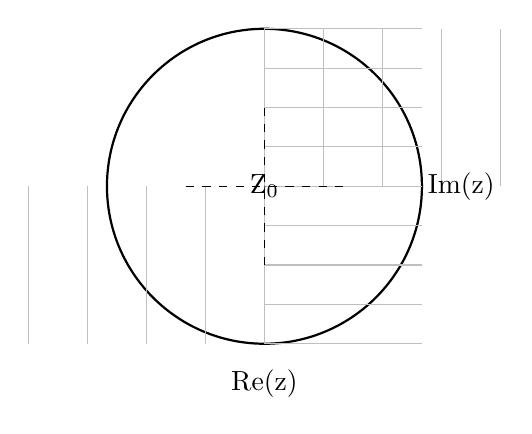
\begin{tikzpicture}
    \draw[thick] (0,0) circle (2cm); % Outer circle
    \foreach \x in {0,0.5,1,1.5,2} {
        \draw[gray!50] (\x*1.5,0) -- (\x*1.5,2);
        \draw[gray!50] ({-\x*1.5},0) -- ({-\x*1.5},-2);
    }

    \foreach \y in {-2,-1.5,...,2} {
        \draw[gray!50] (0,\y) -- (2,\y);
        \draw[gray!50] (0,{-\y}) -- (2,{-\y});
    }

    \node at (0,-2.5) {Re(z)};
    \node at (2.5,0) {Im(z)};
    \node at (0,0) {Z$_0$};
    
    \draw[dashed] (-1,0) -- (1,0); % Mark axis
    \draw[dashed] (0,-1) -- (0,1); % Mark axis
\end{tikzpicture}

This diagram illustrates the real and imaginary axes of the Smith chart where the normalization takes place, allowing the user to visualize impedance transformation effectively.

In summary, when normalizing the Smith chart, one must focus on reassigning the prime center's impedance value to facilitate the analysis of different circuit elements' impedance characteristics. This normalization is a key step in using the Smith chart effectively in radio frequency applications.
